\skriptsection{Spektren}{103}
\skriptsubsection{Spektraldarstellungen}{103ff} 

\begin{figure}[htbp]
  \centering
  \begin{minipage}[b]{5.5cm}
    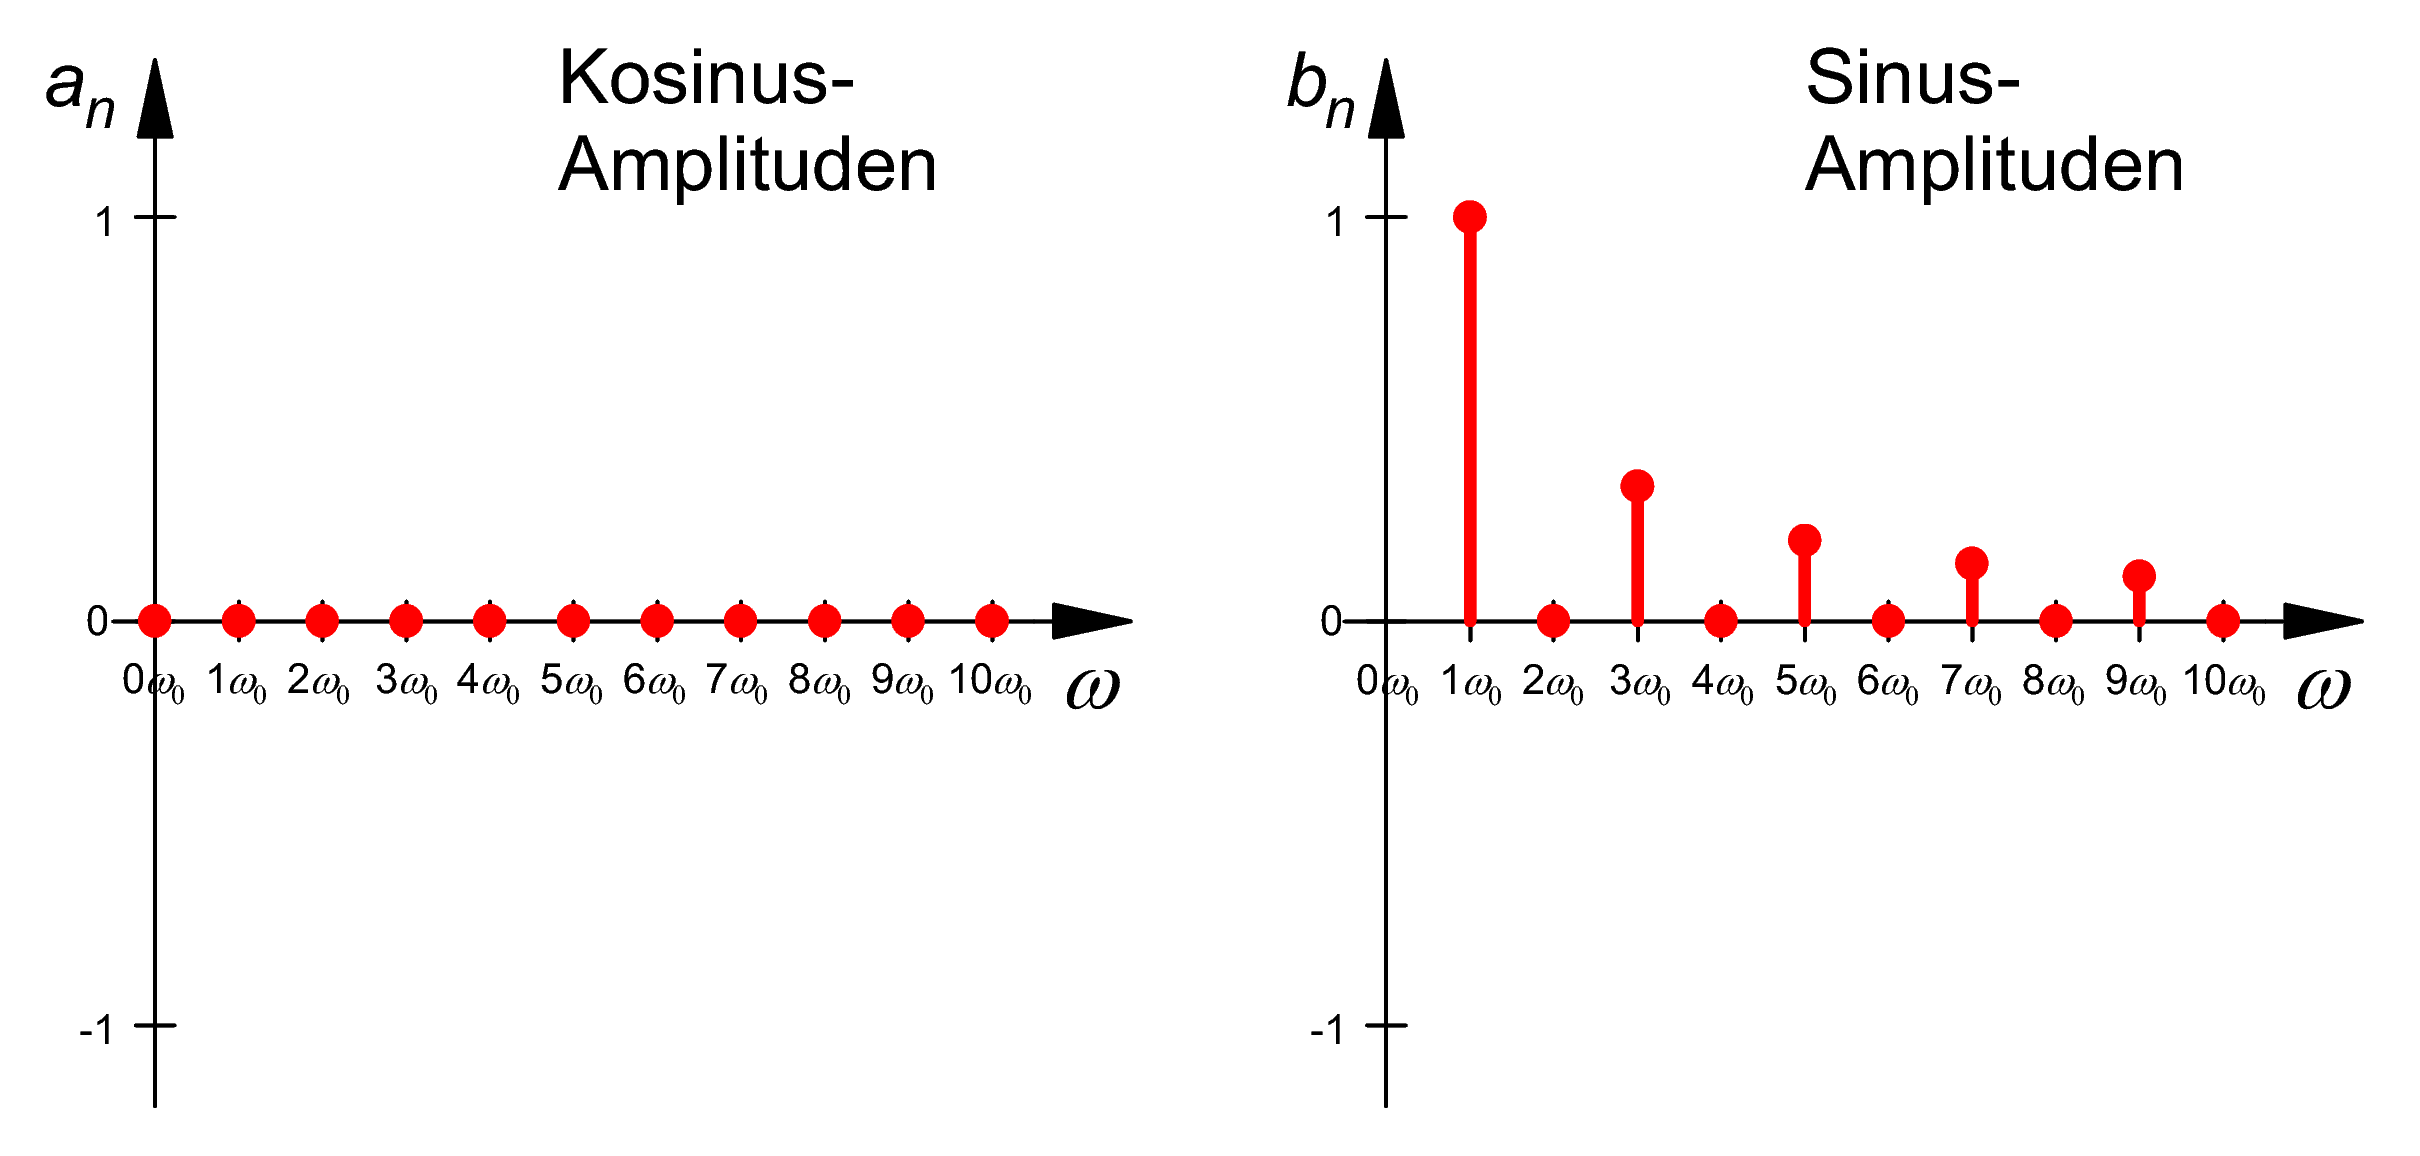
\includegraphics[width=5.5cm]{./bilder/spektren_cossin.png}
    \caption{Kosinus- und Sinusamplitudendiagramm} 
  \end{minipage}
  \hspace{1cm}
  \begin{minipage}[b]{5.5cm}
    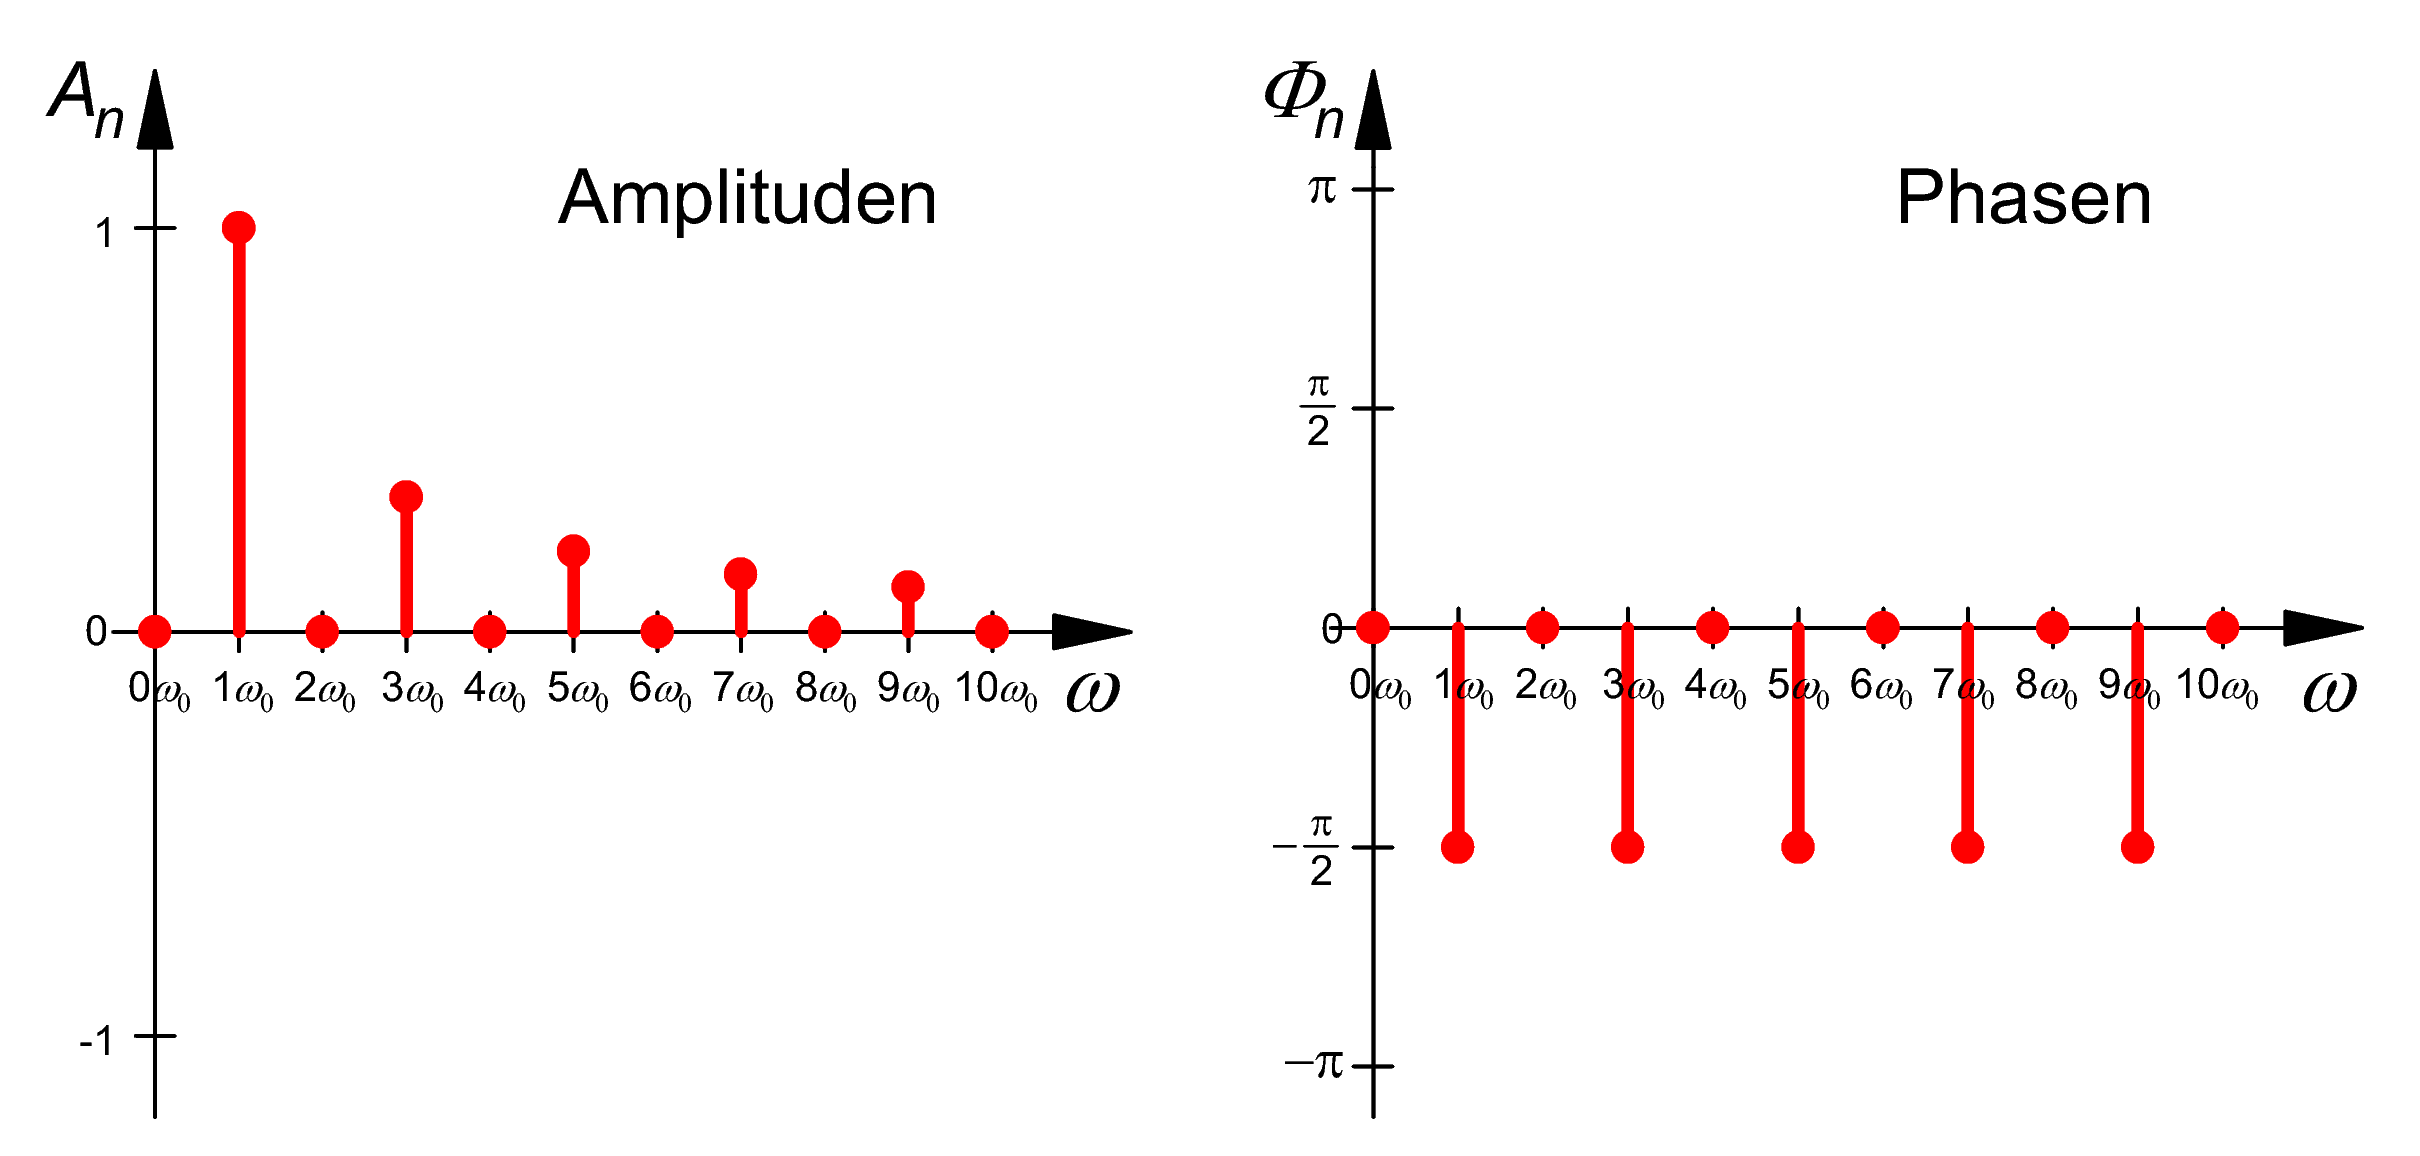
\includegraphics[width=5.5cm]{./bilder/spektren_einseitig.png} 
    \caption{Einseitiges Amplituden-/Phasendiagramm} 
  \end{minipage}
  \hspace{1cm}
  \begin{minipage}[b]{5.5cm}
    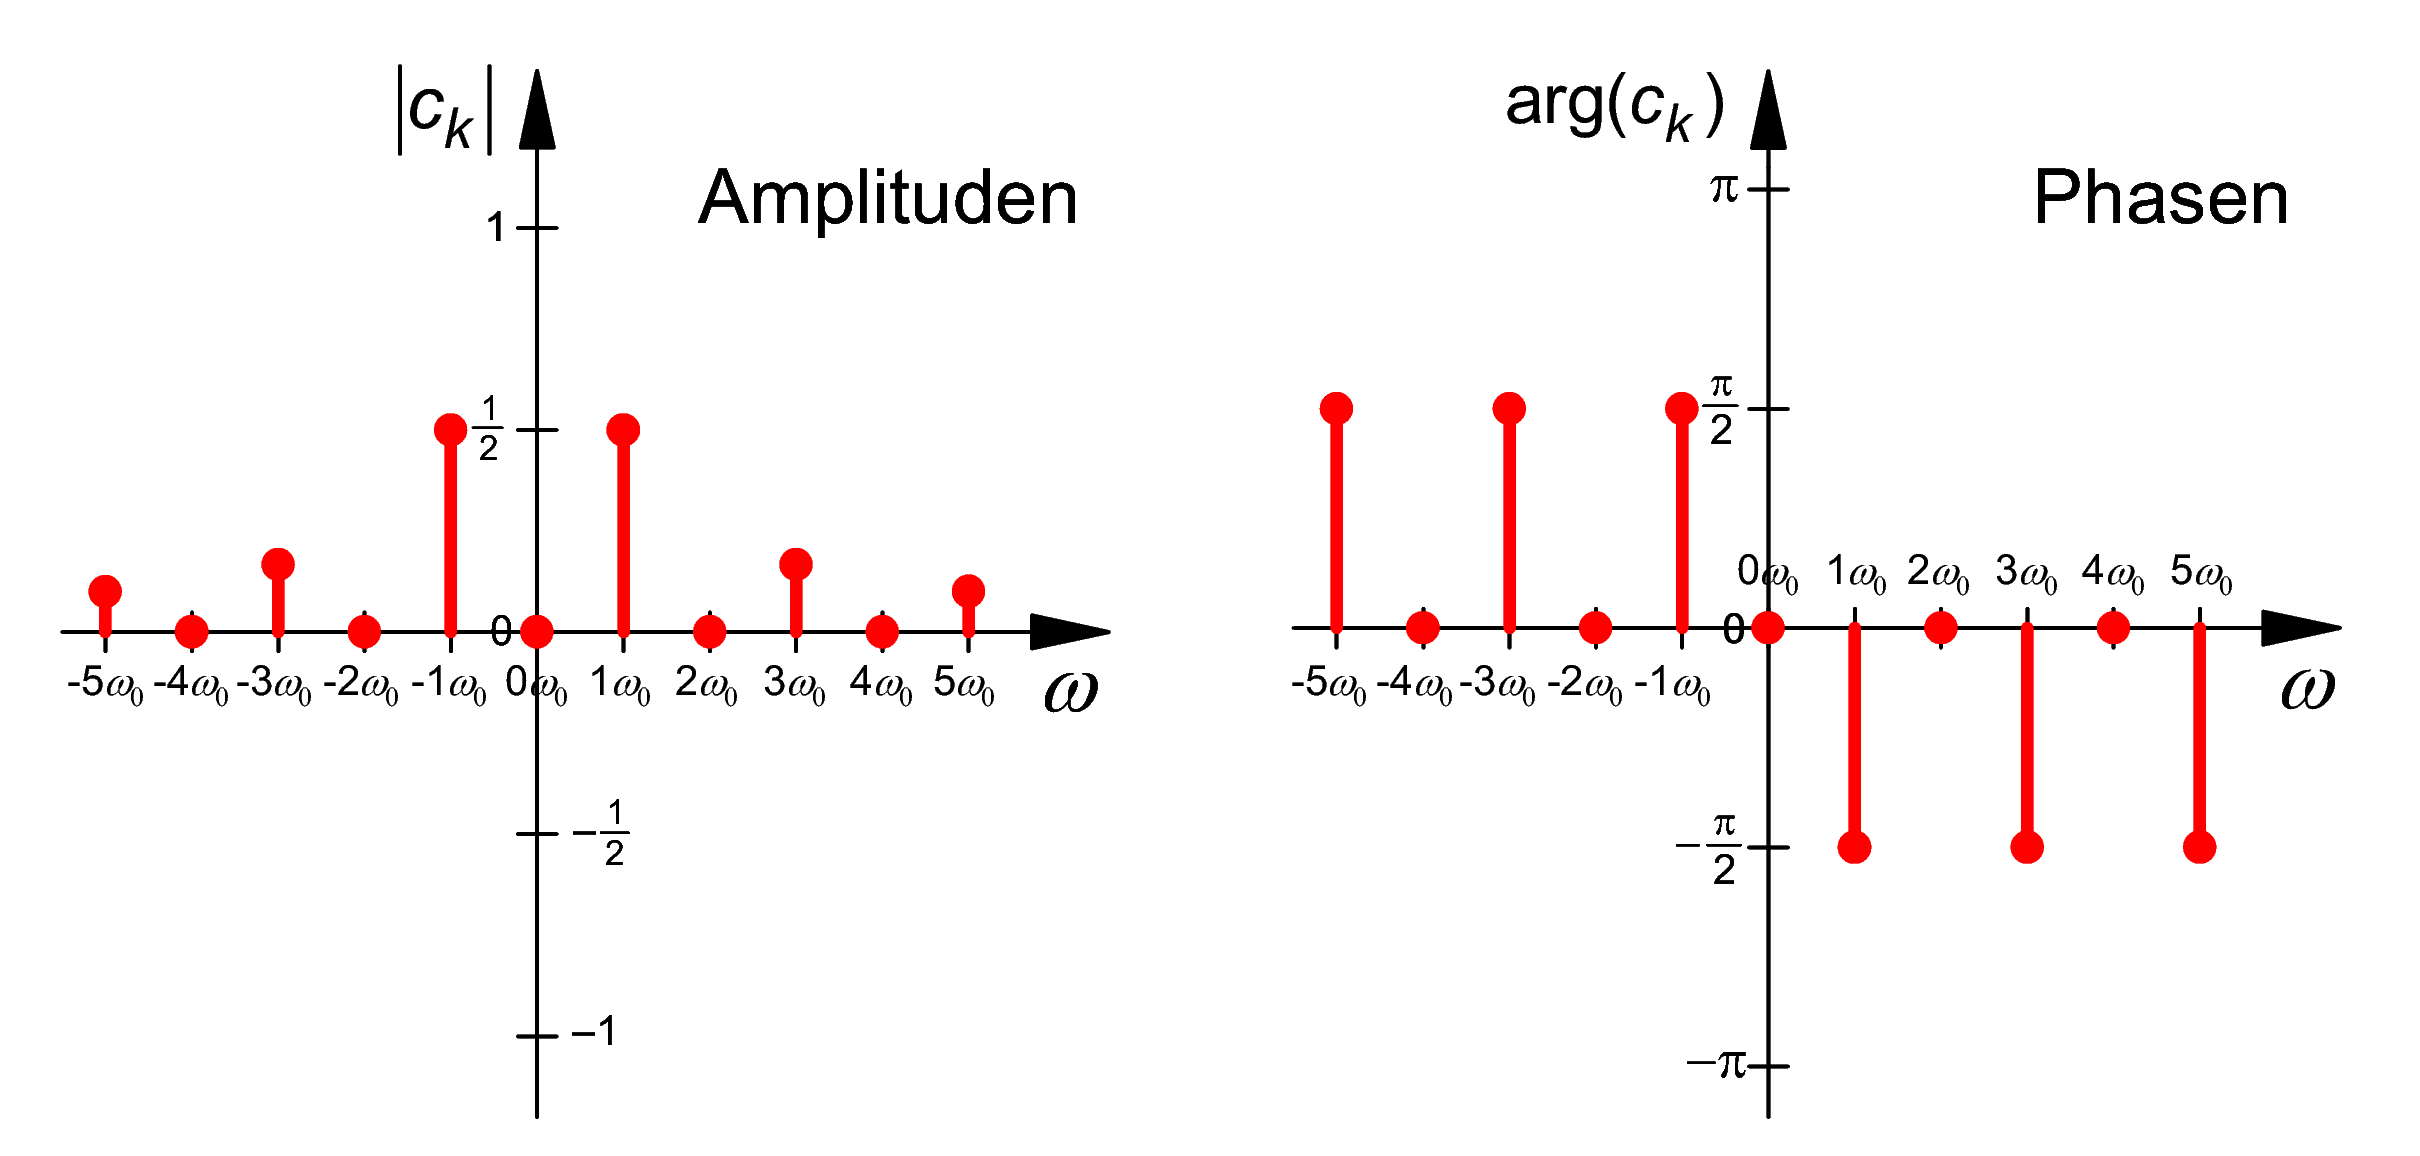
\includegraphics[width=5.5cm]{./bilder/spektren_zweiseitig.png} 
    \caption{Zweiseitiges Amplituden-/Phasendiagramm} 
  \end{minipage}
\end{figure}

\subsubsection{(1) Kosinus- und Sinusamplitudendiagramm} 
Reelle Fourierkoeffizienten ($a_n, b_n$) können direkt abgelesen werden. 
Bei einer Phasenverschiebung ändern sich jedoch die Koeffizienten grafisch nicht nachvollziehbar. \\
Diese Darstellung hat gegenüber den anderen zwei mehr Nachteile und wird daher eher selten genutzt.

\subsubsection{(2) Einseitiges Amplituden-/Phasendiagramm} 
$A_n = |a_n - j \cdot b_n| = \sqrt{a_n^2 + b_n^2}$ \text{ oder } $A_n = 2 \cdot |c_n| \qquad$
$\Phi_n = \arg(a_n - j \cdot b_n) \text{ oder } \Phi_n = \arg(c_n) $ \\
Spezialfall $n=0 \Rightarrow A_0 = |\frac{a_0}{2}| \text{ und } \Phi_0 = \left\{
    \begin{array}{l} 
      0, \quad a_0 \geq 0\\
      \pi, \quad a_0 < 0  
    \end{array}
      \right. $

\subsubsection{(3) Zweiseitiges Amplituden-/Phasendiagramm (komplexes Spektrum)} 
Amplitudendiagramm ist achsensymmetrisch wegen $ c_n=\overline{c_{-n}} $. Phasendiagramm ist punktsymmetrisch. \\
Ähnlichkeit mit Einseitigem: $|c_k| = \frac{1}{2}A_k $ und $\arg(c_k) = \Phi_k$ für alle $ n \geq 0$.

\skriptsubsection{Spezialfälle}{106}
\begin{tabular}{ll}
  Funktion f gerade 
  & (1) Sinusamplitudendiagramm überall 0 \\
  & (2,3) Phasendiagramm enthält nur die Werte $0$ und $\pi$ \\
  Funktion f ungerade
  & (1) Kosinusamplitudendiagramm überall 0 \\
  & (2,3) Phasendiagramm enthält nur die Werte $\pm \frac{\pi}{2}$ (oder $0$ falls Amplitudenwert $=0$) \\
  "Ahnlichkeit $g(t) = f(r \cdot t) $
  & (1,2,3) Das Spektrum von $g$ ist das horizontal mit den Faktor $r$ gestreckte Spektrum vom $f$. \\
  Zeitverschiebung $g(t) = f(t + t_0) $
  & (1) \verweis{Fourier_Zeitverschiebung}{Zeitverschiebung} \\
  & (2,3) Amplitudendiagramme sind identisch. \\
  & (2,3) Phasendiagramme: Die Sälule der Frequenz $k \omega_0$ wächst um $k\omega_0 t_0$. \\
  Weisses Rauschen
  & "Uberlagerung von Schwingungen aller möglichen Frequenzen \\
  & mit gleichen Amplituden und zufälligen Phasen. 

\end{tabular}

\begin{center}
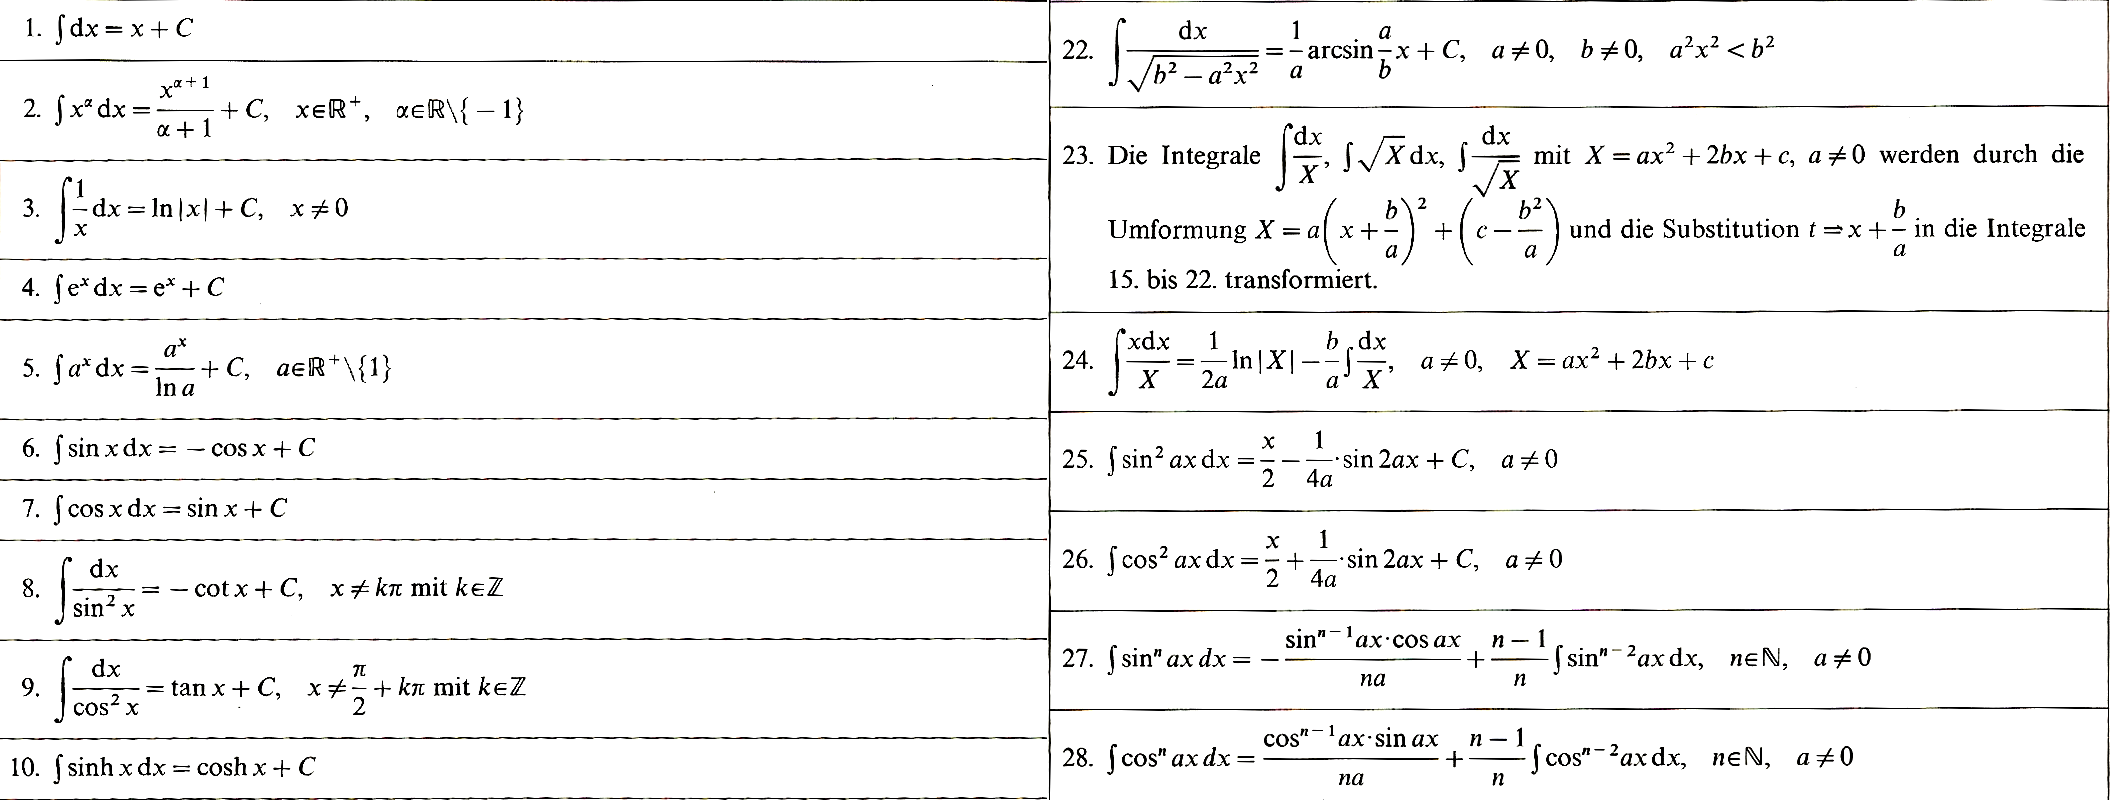
\includegraphics[width=18cm]{./bilder/integral1.png}
\end{center}